\documentclass[]{rsos}
\usepackage{subfigure}
\usepackage{amssymb}
\usepackage{amsmath}
\usepackage{graphicx}
\usepackage{todonotes}
\newcommand{\degree}{$^{\circ}$\ }

\begin{document}


\title{Does pre-crastination explain why some observers are sub-optimal in a visual search task?}

\author{Alasdair D. F. Clarke$^{1}$, Kyle Sauerberger$^{2}$, Anna Nowakowska$^{3}$,\\ David A. Rosenbaum$^{2}$, Thomas R. Zentall$^{4}$ \& Amelia R. Hunt$^{3}$}

\address{$^{1}$Dept. of Psychology, University of Essex, UK\\
$^{2}$Dept. of Psychology, University of California, USA\\
$^{3}$School of Psychology, University of Aberdeen, UK\\
$^{4}$Dept. of Psychology, University of Kentucky, USA}

%%%% Subject entries to be placed here %%%%
\subject{Psychology}


%%%% Keyword entries to be placed here %%%%
\keywords{optimal behaviour, visual search, eye movements}

%%%% Insert corresponding author and its email address}
\corres{A. D. F. Clarke\\
\email{a.clarke@essex.ac.uk}}

% \maketitle
\begin{abstract}
How do we decide where to search for a target? Optimal search relies on first considering the relative informational value of different locations, and then executing eye movements to the best options. But many participants consistently move their eyes to locations that can be easily ascertained to neither contain the target, nor to provide new information about the target's location. Here we ask whether this sub-optimal search behaviour represents a specific example of a general tendency towards \textit{pre-crastination}: starting sub-goals of a task before they are needed, and in so doing, spending longer doing the task than is necessary. To test this hypothesis, we will ask 200 participants to do two tasks: retrieve two heavy buckets (one close and one far), and search for a line segment. Pre-crastination is defined as consistently picking up the closer bucket first, versus the more efficient strategy of picking up the farther bucket first. Search efficiency is the proportion of fixations directed to more cluttered regions of the search array. We predict an association of pre-crastination with inefficient search strategies. Personality inventories will also be administered to identify stable characteristics associated with these strategies. 
\end{abstract}

\begin{fmtext}


Human behaviour in visual search tasks is characterised by large individual differences. While both optimal \cite{najemnik-geisler2008,hoppe-rothkopf2019} and stochastic \cite{clarke2016} strategies have been proposed, 
\end{fmtext}
\maketitle
experiments show that different observers utilise different strategies \cite{nowakowska2017,irons-leber2016}, with some approximating the optimal search strategy, others behaving randomly, and others still, making use of a `counter-optimal' strategy. The challenge for a complete understanding of visual search is to identify the source(s) of these individual differences.


In the \textit{split-half} visual search paradigm \cite{nowakowska2017}, the observer is presented with a stimulus similar to that shown in Figure \ref{fig:stimulus}. The observer's task is to decide whether the target (a line segment oriented $45^{\circ}$ to the right) is present or not, as quickly and accurately as possible. One side of the display contains distractors of a similar orientation, and the other contains more variable orientations. In this situation the optimal strategy is to use central vision to search the side of the stimulus containing the heterogeneous orientations: were the target present on the more homogeneous side of the display, the observer would be able to use peripheral vision to see it immediately. Moving the eyes towards the homogeneous side provides no new information and slows down search considerably (indeed, in \cite{nowakowska2016}, each fixation on the homogeneous side was estimated to slow response times by 360ms). While approximately a third of observers implement an optimal strategy, a similar number pursued the opposite strategy and searched the easy (homogeneous) side of the display first, despite this leading to slower response times.

\begin{figure}
\centering
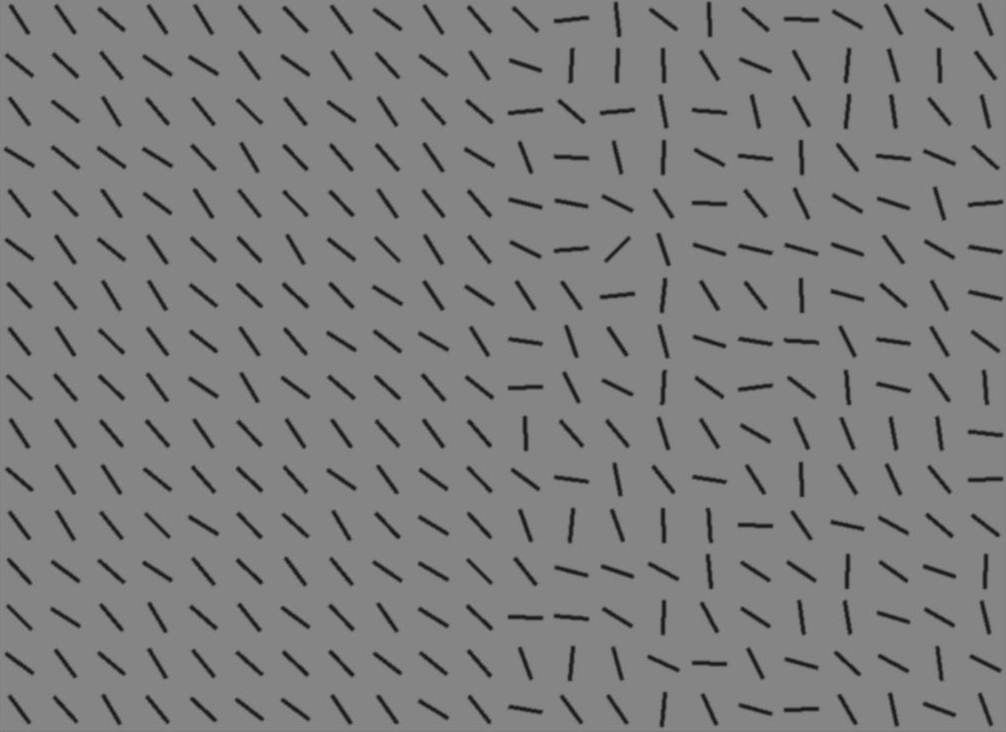
\includegraphics[width=6cm]{Figures/split-half.png}
\caption{An example of the split-half line segment stimuli. The target is the unique line segment oriented $45^{\circ}$ to the right. Participants who direct their saccades to the heterogeneous half of the display are faster to correctly respond target absent/present than those who fixate the homogeneous half of the display.}
\label{fig:stimulus}


\end{figure}

Departures from optimality have also been found in other visual search tasks, such as Irons \& Leber's \cite{irons-leber2016,irons-leber2018} task, in which two unique targets are present and participants need to find only one of them. Predictable changes to the distractors make one target easier to find than the other. A subset of participants showed optimal performance, in that they searched for the easier target, given the set of distractors on that trial. But the majority of participants did not switch between targets in a way that was related to changes in the distractors. Curiously, while both of the Irons \& Leber and split-half line segment paradigms appear to have good test-retest correlations ($r \approx 0.75$), there is at best only a weak correlation between the two \cite{clarke2019}. This suggests that it is not the case that some people are ``good at looking for things'' while others are not. Instead, something about the structure of the particular task leads some people to perform well and others to perform badly.

Previous attempts have similarly failed to link behaviour during visual search tasks with broader personality and individual difference measures. Irons \& Leber found no correlation with search strategy for working memory, impulsiveness, novelty-seeking, intolerance of uncertainty, or need for cognition\footnote{There was a small, statistically significant correlation between need for cognition and switch rate.} \cite{irons-leber2016,irons-leber2018}. Similarly, J{\'o}hannesson et al. found no evidence of an effect of working memory or inhibitory control on foraging behaviour \cite{johannesson2017}. Given that these search tasks appear to uncorrelated, a general trait is unlikely to explain variability in all search tasks.  

In the present study, we investigate the hypothesis that participants who are sub-optimal in our split-half line segment search task have a tendency towards \textit{pre-crastination}, a phenomenon where participants prioritise the completion of a sub-goal, even if it results in extra effort overall \cite{rosenbaum2014}. In the original study, participants were asked to walk down a corridor, pick up one of two heavy buckets as they passed, and carry it to the finish line. The two buckets were placed at different distances between the start and finish line, and the optimal (in terms of minimising effort) strategy is to pick up the bucket that is furthest from the starting position and closer to the finish line. Despite this simple solution, most participants favoured picking up the first bucket they came to, even though that resulted in them having to carry it further. This tendency was named \textit{pre-crastination}, and has since been replicated several times in both humans \cite{fournier2019task} and pigeons \cite{wasserman2015}. In an even more dramatic version of the task, Fournier and colleagues (2019) asked participants to go get two buckets - one close and one further away - and bring them back to set them on a table behind them. The majority (36 out of 49 participants in the key condition) chose to pick up the close bucket first, carry it out to the further bucket, and then bring both back, even though this order is clearly more effortful than picking up the far bucket and then grabbing the close one on the way back to the table.

As a first step to assessing our hypothesis, we conducted a pilot study to ensure we would replicate the variability between participants in a shorter version of the search task, and that we could clearly classify people into two groups based on whether they pick up the close bucket first (i.e. "pre-crastinators") or the farther bucket (optimal). The pilot data were also intended to be used to refine our approach to data processing, visualization, and analysis. Both of the previous findings (search variability, \cite{nowakowska2017}, and pre-crastination, \cite{fournier2019task}) were clearly replicated in the pilot experiment. Surprisingly, the data suggested a relatively robust relationship between pre-crastination and visual search strategy, but in the opposite direction to the one which we originally expected, with pre-crastinators having a tendency to search more efficiently rather than less. We therefore revised our aim to be more data-driven than the original hypothesis, aiming to estimate the variability in search performance accounted for by pre-crastination. The pilot data also suggested that the relationship between pre-crastination and visual search may by mediated by differences in speed-accuracy trade-offs between participants, so we plan to explore this aspect of visual search as well.  

If we confirm the existence of a relationship between these two tasks, a natural question is whether this can be accounted for by personality traits of the individuals.  A personality trait is an enduring pattern of thoughts, feelings, and behaviours that is stable across time and contexts \cite{funder2016}. Previous research suggests that those who precrastinate are motivated, responsible, and energetic \cite{rosenbaum2019}. Specifically, \cite{sauerberger2019} found a correlation of $r = 0.22$ between precrastinaion and  conscientiousness, which we will attempt to replicate. Speculatively, these traits may also cause participants to search in a more thorough, but less efficient, manner, aligning with the interpretation that precrastinating, although costly, may not be irrational to the degree that participants prefer maximizing thoroughness over maximizing efficiency. Examining personality traits in this study will help to further uncover the individual difference factors associated with precrastination and different visual search strategies. 

Our experiment tests the hypothesis that pre-crastination might represent a rational approach to doing tasks, i.e., a reasonable tendency to get the difficult part of the task out of the way first. If precrastination is positively related to efficient search, this would be evidence in favour of a ``rational'' interpretation of precrastination, as opposed to the alternative interpretation that it reflects an irrational impulse to grab the closest task-related object (in which case, a negative correlation with search efficiency would be more likely). In addition, the experiment has the potential to assess whether the already-established link between pre-crastination and conscientiousness could generalize, and be a potential explanation for the wide range of different search strategies previously observed. This would have important implications for theories of visual search, which tend to make assumptions about how ''people'' (as a group) direct their eyes during search; if personality traits can be directly predictive of eye movement strategies, this will challenge the field to more carefully refine its assumptions. In addition to the clear theoretical contribution our results could have, they could also illustrate that efficient/optimal tendencies in one circumstance can translate to inefficient choices in others. Finally, we have noticed in many fields that there is a lack of correlational studies relating behavioural measures to each other (as opposed to relating behavioural measures to personality traits).

\section{Pilot Results}

Data from 30 participants were analysed as part of our pilot study. These were classed as either pre-crastinating ($n=13$) or not ($n=17$) based on their behaviour in the bucket task, as described in Section \ref{sec:pre-crastination_methods}. We now investigate the extent to which this classification of participants is correlated with the variance observed in the split-half visual search task.

\subsection{Accuracy and Reaction Time}
Each participant's median reaction time and accuracy was computed for the split-half visual search task, presented in Figure \ref{fig:exp1_summary}. It appears that the group of participants who pre-crastinated in the bucket task found fewer (median accuracy of 0.33) of the hard targets in the visual search task than the participants who did not pre-crastinate (median 0.46). We can also see that the pre-crastinators had shorter median response times: \textit{easy}: 0.99 v 1.03 seconds; \textit{hard}: 6.71 v 8.91 seconds; and \textit{absent}: 8.08 v 9.95 seconds. These results suggest varying speed-accuracy trade-offs between our two groups, with participants labelled as pre-crastinators being more likely to give up before finding the hard targets. 

\begin{figure}[t]
  \centering  
  \subfigure[]{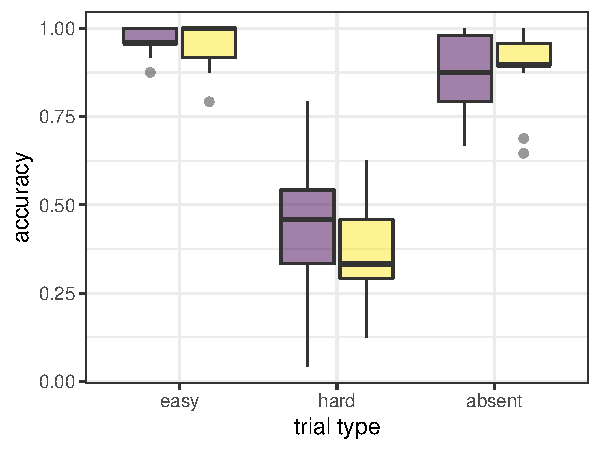
\includegraphics[width=6cm]{../pilot_experiment/scratch/acc.pdf}}
  \subfigure[]{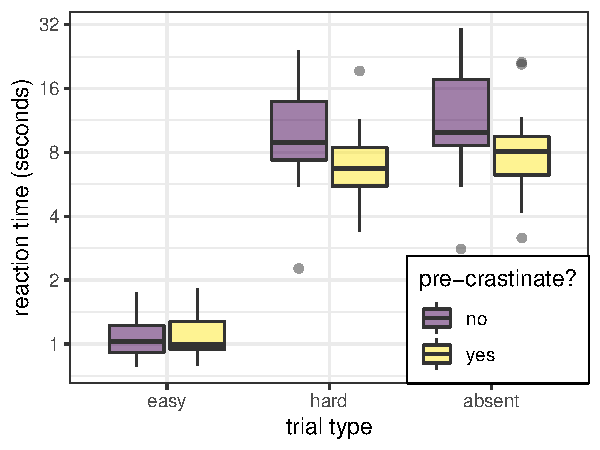
\includegraphics[width=6cm]{../pilot_experiment/scratch/rt.pdf}}
  \caption{The distribution of (a) accuracy and (b) reaction time measures in the split-half visual search task. Note that the $y$-axis for (b) has been $\log_2$-scaled. Dots represent points classed as outliers, defined as being below or above $1.5 \times$ the inter-quartile range away from the first or third quartile.}
  \label{fig:exp1_summary}
\end{figure}

\subsection{Search Strategy}
To investigate the relation between a participant's tendency to pre-crastinate and how they approach the visual search task, we fit beta distributions\footnote{a distribution that is bounded by (0,1) and hence suitable for modelling proportions.} to the strategy metric for each group. The strategy metric is defined as the proportion of fixations two-through-five directed to the heterogeneous half of the display. We use a Bayesian approach with a conservative prior for the difference in group means. We assume that the mean of each group is 0.50, with a $95\%$ highest posterior density interval (HPDI) $= [0.27, 0.73]$. Our prior for the difference between groups is conservative, $\beta \sim\mathcal{N}(0, 0.50)$, which gives a distribution with a $95\%$ HPDI $=[-0.047, 0.046]$. These distributions are illustrated in Figure \ref{fig:exp1_strategy}(a).

After conditioning the model on the data, we obtain posterior probability distributions shown in Figure \ref{fig:exp1_strategy}(b). Our best estimate for the difference in group means is 0.125, with a $95\%$ HPDI of $[-0.003, 0.242]$. An alternative summary would be that $p(\delta >0 | X)  = 0.973$\footnote{Comparing the frequentist approach to our Bayesian model, we can see that a $t$-test gives both a less precise, and more positive, estimate of the difference: $t=2.66$, $df = 27.5$, $p=0.013$, $95\%CI = [0.04, 0.32]$.}.

\begin{figure}[t]
  \centering  
  %\subfigure[]{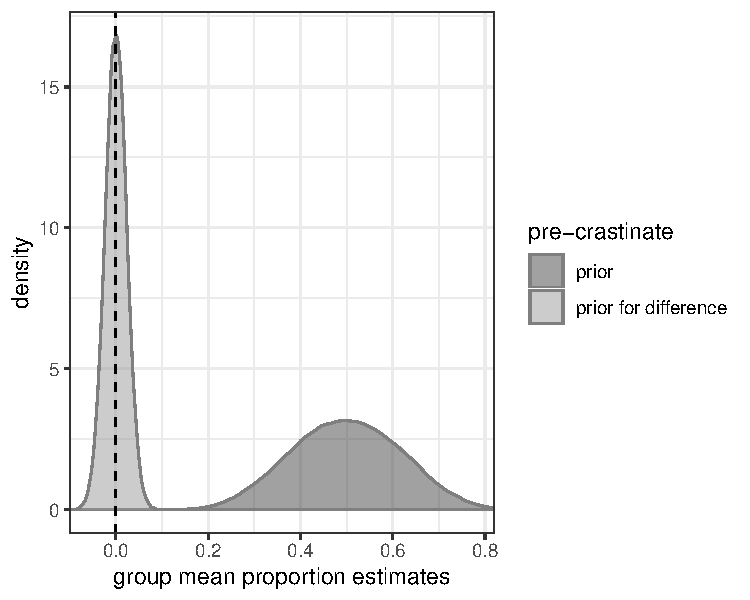
\includegraphics[width=6cm]{../analysis/scratch/pilot_prior_plot.pdf}}
  %\subfigure[]{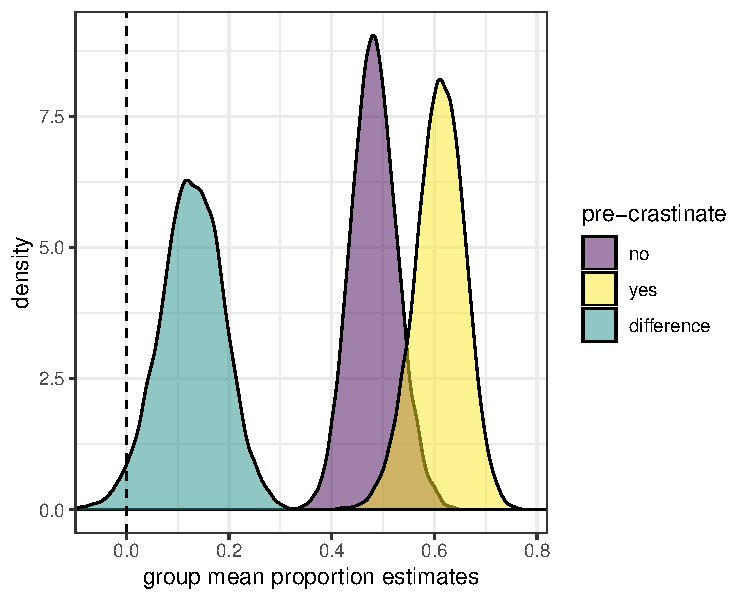
\includegraphics[width=6cm]{../analysis/scratch/pilot_plot.pdf}}
  \caption{(a) Prior and (b) posterior distributions for the mean of the two groups of participants, and the difference between them. Our priors for the two groups are identical, hence the overlapping distributions.}
  \label{fig:exp1_strategy}
\end{figure}

\subsection{Discussion \& Hypotheses for Registration}

Based on the results of our pilot analysis, it appears that there is a relationship between pre-crastination and visual search strategy: participants who did not pre-crastinate had a mean value of 0.5 for their strategy metric, while those who did pre-crastinate searched more optimally, with a mean strategy metric of around 0.625. Interestingly, this goes against our original intuition in which we viewed pre-crastination as sub-optimal behaviour, that may explain the sub-optimal behaviour in our search paradigm: people who needlessly pick up the closer bucket would be the same people who needlessly search the homogeneous half of the display. The pilot data supports the opposite conclusion: sub-optimal pre-crastination leads to more optimal behaviour in our visual search task. Upon reflection, participants who show a desire to start their task sooner may be starting the search task sooner as well, by targeting the heterogeneous regions where effortful search is required. If confirmed, this relationship would reinforce the interpretation that precrastination does not indicate suboptimal decision strategies, but instead indicates a conscientious approach to task performance.

As such, we will investigate the following hypotheses:

\begin{enumerate}
\item There is a difference (in either direction) in search behaviour between those participants who pre-crastinated and those who did not. This will be determined by looking at \textcolor{red}{$p(\lvert \delta \rvert >0.05 | X)$. A value >0.95 will be taken as evidence of a difference.} 
\item The magnitude of the difference is in-line with the value of 0.125 ($95\%$ HPDI of $[-0.003, 0.242]$) obtained in our pilot experiment. This will be determined by comparing the new HPDI with the pilot HPDI. A new estimate for the size of the difference will then be computed by pooling all data in a mixed-effect model (with random effects for data collected in Aberdeen, Essex, and Pilot).
\item There is a positive correlation ($r=0.22$) between pre-crastination and conscientiousness.
\end{enumerate}

\section{Methods}

We will recruit 200 participants for this experiment. This large sample size is due to the addition of personality measures: Larger samples provide greater power to detect the typical effect sizes in those fields, reduce Type I error, and increase the chances of replicable findings \cite{fraley2014}. Participants will be recruited via participant panels and opportunity sampling at the universities of Aberdeen and Essex. The protocol has been approved by the ethics committees at both universities. Participants will complete the bucket-retrieval task both before and after the visual search task, so no counterbalancing will be needed. Additional participants will be recruited to replace any who are excluded from data analysis (details below). 

A one-tailed correlation power analysis (using the \texttt{pwr} package \cite{pwr}) with $\alpha=0.05, \beta=0.8$ and $n=200$ gives $r=0.175$.

\subsection{Pre-crastination}
\label{sec:pre-crastination_methods}
\subsubsection{Apparatus \& Stimuli}

Figure \ref{fig:buckets} is a photograph of the bucket task set-up. Two 10 litre buckets will be filled with sand until the total weight of each bucket is 3kg. The experiment will take place in a quiet corridor. Buckets will be placed at 6ft and 16ft away from the start position, which is marked as a T with green tape. Buckets will be placed on crates at about hand height. Just behind the start position is a pair of crates on which to set the buckets down to end the trial.

\begin{figure}
\centering
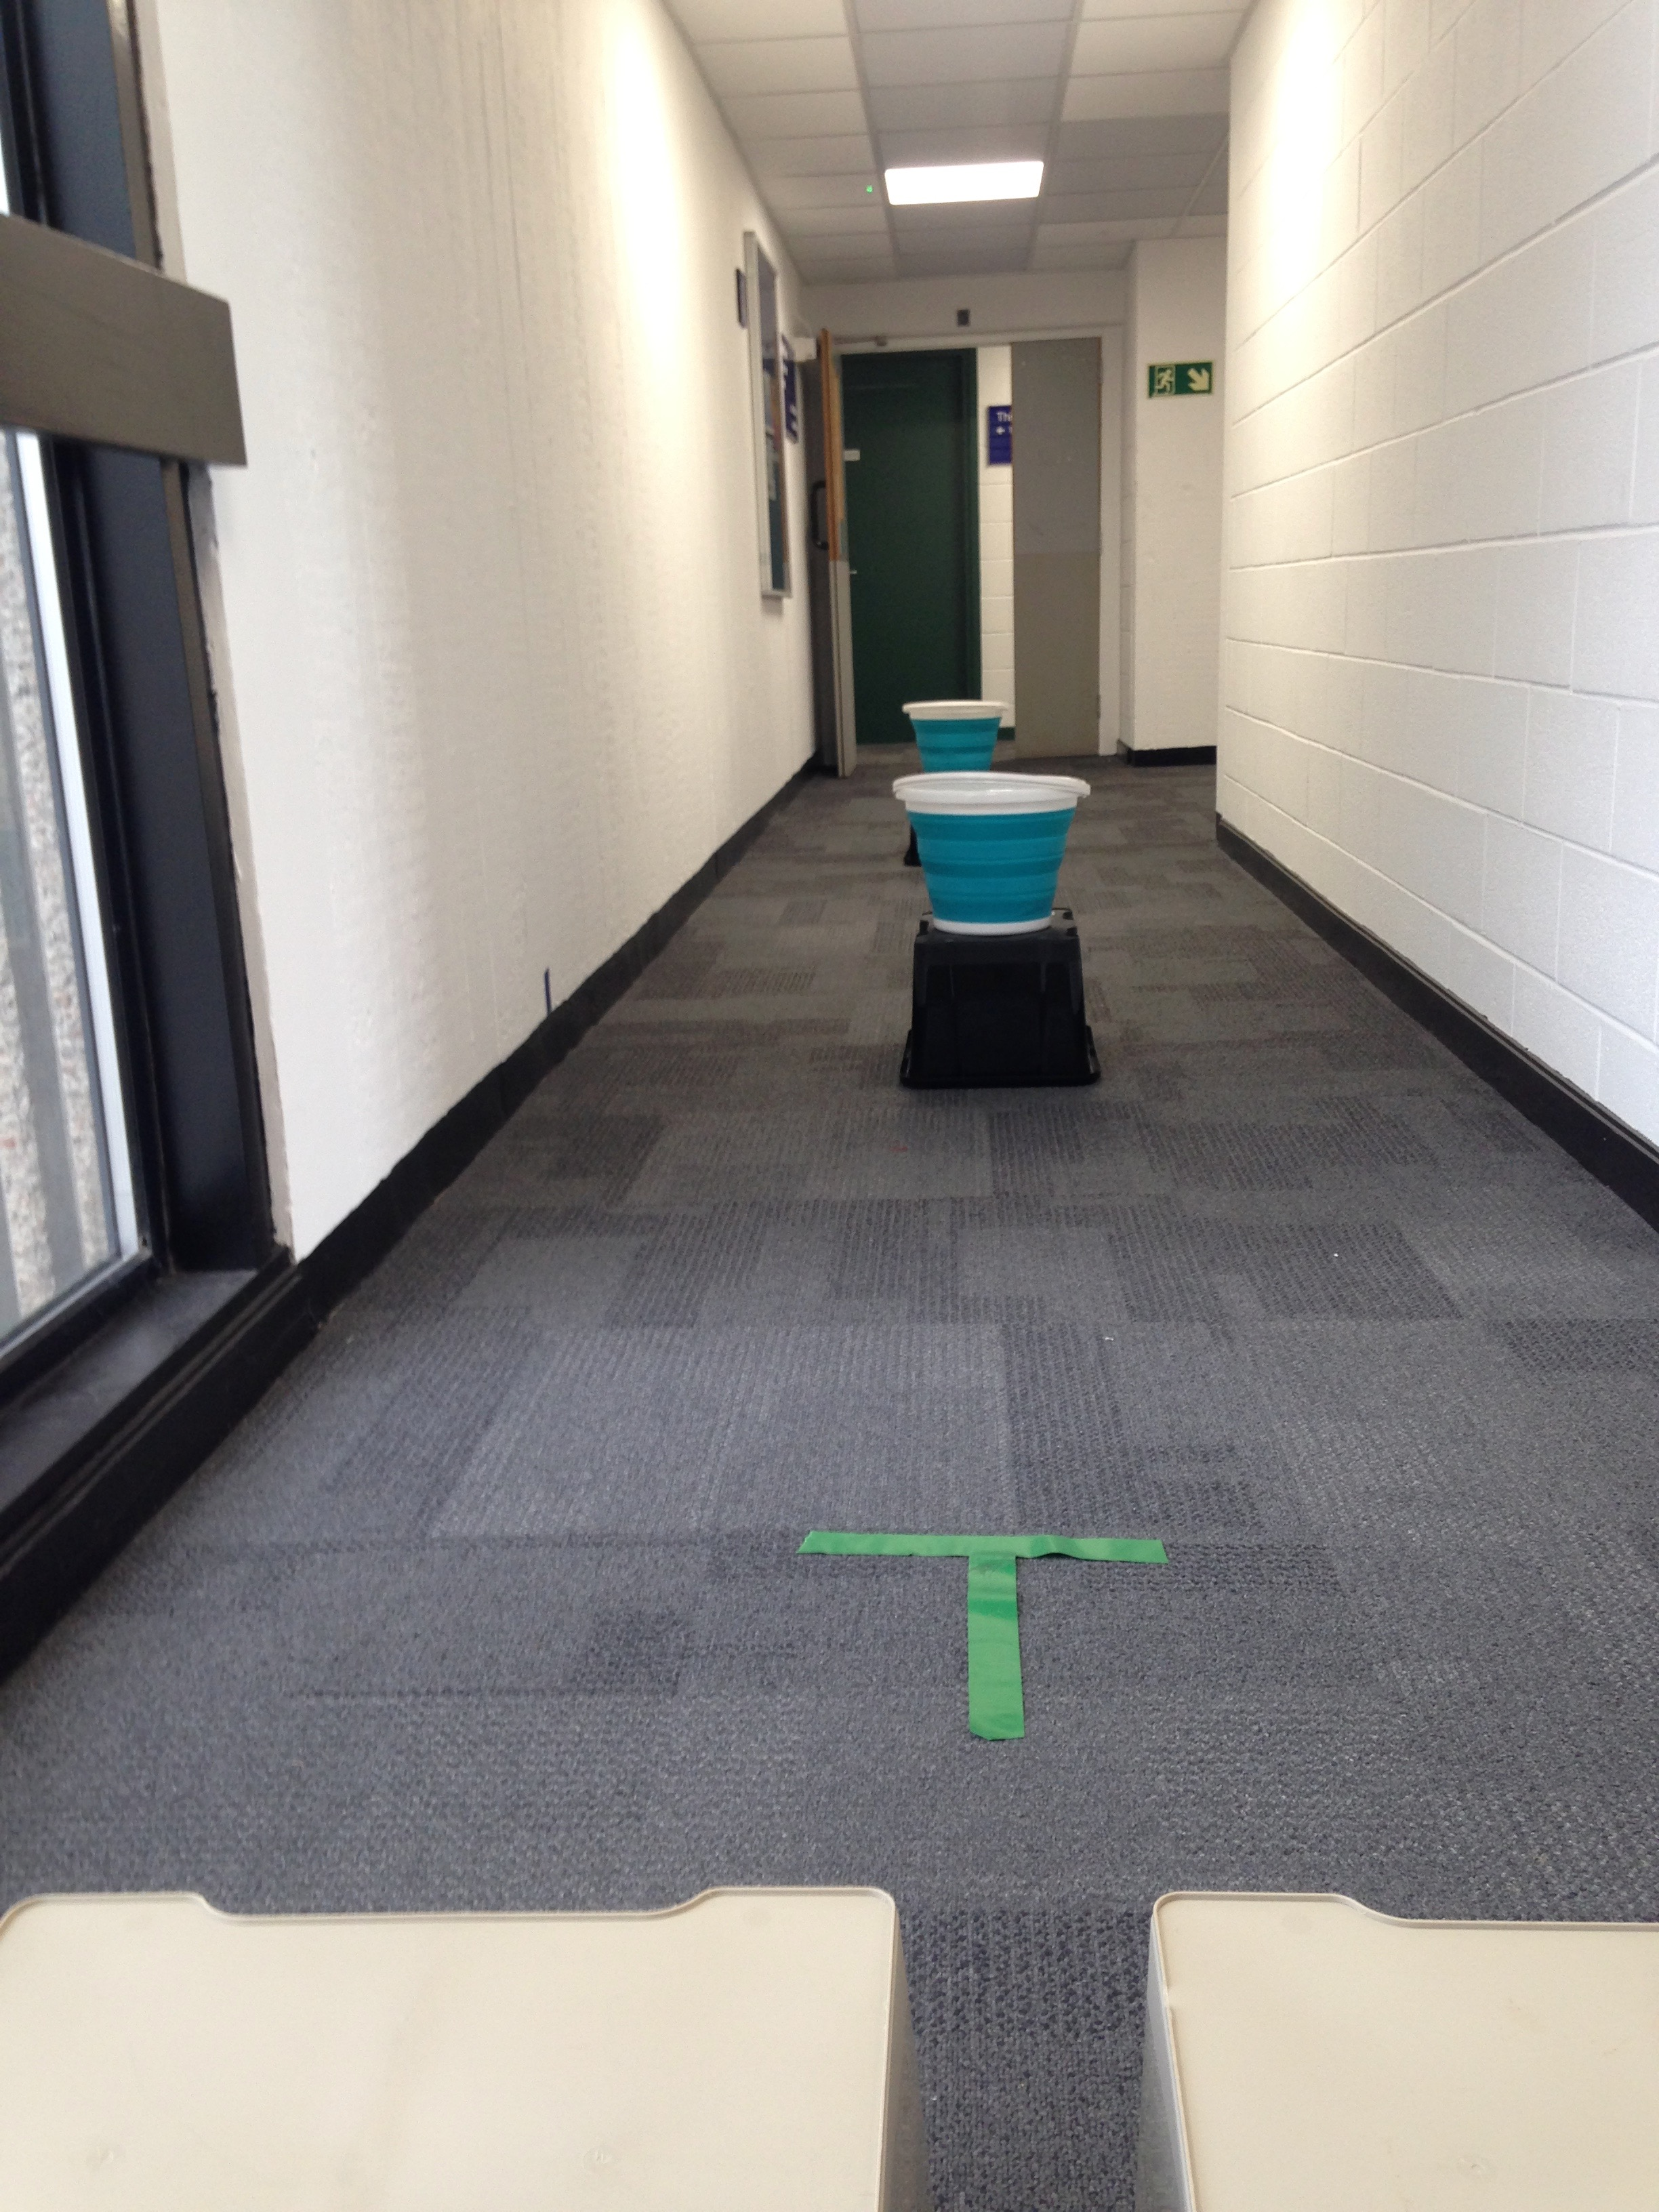
\includegraphics[width=6cm]{Figures/IMG_7939.jpg}
\caption{Set-up for the pre-crastination part of the experiment.}
\label{fig:buckets}
\end{figure}

\subsubsection{Procedure}

The task replicates that used in \cite{fournier2019task}, in which participants were instructed to pick up two buckets and place them on the crates behind the start position. We will closely follow the methods and instructions as described in their appendix. Each participant will complete three trials before the visual search task, and three trials after. While the experimenter is setting up the buckets for the next trial, the participant will be asked to walk over to a nearby window and look outside until they are asked to return. The full protocol and instructions given to participants is available at <insert url here>. 

\subsubsection{Data processing}

Participants will be classified as "pre-crastinators" if they pick up the closer bucket first, and "optimal" if they pick up the far bucket first. Based on the pilot data, and that of \cite{fournier2019task}, we expect the results from the bucket task to be largely binary, with participants picking up either the close or the far bucket on every trial. If the data are similarly binary in this experiment, we will continue to treat pre-crastination as a two-level categorical factor. Participants who pick up the closest bucket on at least five of the six trials will be classed as pre-crastinators, while those who pick up the closest bucket on no more than two out of six trials will be non-pre-crastinators. Participants with intermediate behaviour will be excluded. 

There is also a chance that, unlike \cite{fournier2019task}, our sample of participants give rise to a larger range of intermediate behaviours. If more than $25\%$ of our participants would be excluded under the coding scheme outlined above, then we will treat our pre-crastination measure as a three-level factor (if a clear classification is apparent). In this case, the same Bayesian beta regression model will be fit to the data. 

\subsection{Split-Half Visual Search}

\subsubsection{Apparatus \& Stimuli}

Stimuli will be presented on a 17 inch CRT monitor with a resolution of $1024 \times 768$. Stimulus generation, presentation and data collection are controlled by Matlab and psychophysics toolbox \cite{brainard1997,cornelissen2002} run on a mac pro computer. The position of the right eye will be recorded using a desktop-mounted EyeLink 1000 eye tracker (SR Research, Canada) sampling eye position at 1000Hz. 

We will use the same arrays of line segments as in \cite{nowakowska2017} (see Figure \ref{fig:stimulus}). These arrays consist of 22 column and 16 rows on a uniform grey background. The target line is always tilted $45^{\circ}$ degrees to the right, while the mean distractor angle is perpendicular at $45^{\circ}$ degrees to the left. Search difficulty will be manipulated by sampling from either a narrow $30^{\circ}$ range of distractor line orientations (homogeneous) or a wide $106^{\circ}$ range (heterogeneous). Half of each search array consists of homogeneous line segments, while the other half is heterogeneous. Which side is heterogeneous will be randomly determined on each trial. We will use 96 search trials in total, half of which will contain a target. This number of trials was selected based on simulating the results of shorter experiments using the data from \cite{nowakowska2017} (see Figure \ref{fig:num_trials}). The target could be located in any of the possible locations apart from the middle four vertical columns.

\begin{figure}
\centering
 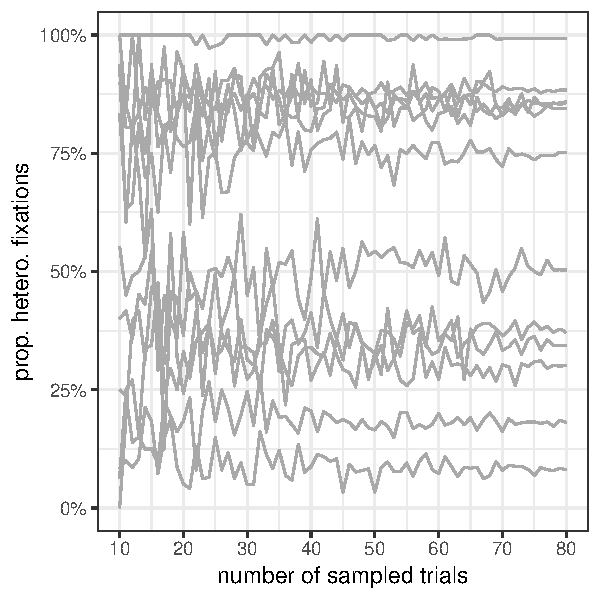
\includegraphics[width=5cm]{Figures/using_smaller_sample_sizes.pdf}
\caption{The effect of reducing the number of target absent trials on measurement accuracy. Each line represents one of the participants from \cite{nowakowska2017}, and at the far right, we can see the measurement of their strategy based on all 80 target absent trials. If we only use a random sample of 48 trials per participant, then we still obtain approximately the same proportion.}
\label{fig:num_trials}
\end{figure}

\subsubsection{Procedure} Before the start of the visual search experiment, participants will undergo a nine-point calibration sequence. Following this, participants will be instructed to report, as quickly as possible, whether a line tilted $45^{\circ}$ to the right was present or not, using the up (present) or down (absent) arrow key. Each search trial begins with a black fixation point (letter \texttt{x}) subtending $1.5\times 2.5$cm ($1.9^{\circ}\times 3.1^{\circ}$), presented at the centre of the computer screen. On the press of a space bar, the stimulus is displayed until the participant makes a response (or times out after 60 seconds). Auditory feedback in the form of a beep, and a 2s red screen, immediately follows incorrect key presses. A set of 8 practice trials precedes the experimental trials.

\subsubsection{Data processing}

Data from participants who fail to achieve at least $75\%$ accuracy for \textit{easy} and \textit{absent} conditions will be excluded as it suggests that they did not understand the task. Fixations during trials will be classified as falling on the homogeneous or heterogeneous half of the display, with fixations falling within the central four columns of line segments being excluded. Following \cite{nowakowska2017} we will summarise each participant's strategy as the proportion of fixations two through five falling on the heterogeneous side of the display during target absent trials. Trials with fewer than five fixations will be excluded, and we will only analysis data from participants who have at least 10 trials. 

\subsection{Personality Questionnaires}

\subsubsection{Materials}

We will administer three personality questionnaires. The first questionnaire is the second iteration of the Big Five Inventory (BFI-2 \cite{soto2017}). The BFI-2 measures five broad personality traits: extraversion (e.g., ``is outgoing, sociable''), agreeableness (e.g., ``has a forgiving nature''), conscientiousness (e.g., ``is efficient, gets things done''), negative emotionality (e.g., ``can be tense''), and open-mindedness (e.g., ``is fascinated by art, music, or literature''). Based on previous research, we suspect that precrastination will have the strongest relationship with conscientiousness. Those who are high in conscientiousness are organised, productive, and responsible, and may have an urge to pick up a bucket as soon as possible.

The second personality questionnaire is the Barratt Impulsiveness Scale (BIS-11 \cite{patton1995}). The BIS-11 measures overall impulsiveness, as well as three subtypes: attentional impulsiveness (``I don't `pay attention'''), motor impulsiveness (``I act on the spur of the moment''), and non-planning impulsiveness (``I say things without thinking''). Based on previous research, we suspect that neither impulsiveness nor its subscales will be related to precrastination.

The third questionnaire is the procrastination scale \cite{lay1986}. The procrastination scale was created specifically for use in student populations and measures a broad range of procrastination behaviours. Sample items include ``I often find myself performing tasks that I had intended to do days before'', ``I generally delay before starting on work I have to do'', and ``I usually have to rush to complete a task on time''. Procrastination is delaying a task or decision with the knowledge that doing so will impair progress towards a goal; it is irrational. Therefore, pre- and pro-crastination should be unrelated.

\subsubsection{Procedure}

PPersonality questionnaires will be administered to participants at the end of the experiment to prevent them from influencing the behavioural measures. Questionnaires will be hosted on Qualtrics and participants will access the questionnaires using a laboratory computer.

Participants will be allowed to skip questions they do not wish to answer. For any one questionnaire, a response rate of less than $75\%$ of questions, or giving the same response for more than $75\%$ of all questions, will invalidate the data from that questionnaire. Participants will be replaced if they answer less than $75\%$ of the questions on the conscientiousness scale (the others are exploratory).

\subsection{Planned Analysis}

The aim of this experiment is to determine if there is a relationship between pre-crastination and the sub-optimal behaviour we observe in the split-half visual search task. Following \cite{nowakowska2017, clarke2019}, each participant's strategy will be represented by the proportion of fixations two-through-five directed to the difficult half of the search area. We will use a Bayesian approach to estimate the extent to which performance in the pre-crastination bucket task is predictive of visual search strategy. Our approach to Bayesian modelling will follow the advice given in \cite{mcelreath2016}, with models fitted using R \cite{r2019} and Stan \cite{carpenter2017stan}. 

As our independent variable is a proportion, we will fit a model using beta regression \cite{ferrari2004beta} with a logit link for for $\mu$ (mean) and a log link for $\phi$ (precision). We will use conservative priors: $\beta \sim\mathcal{N}(0, 0.50)$ and $\gamma \sim\mathcal{N}(0, 1)$ (where $\beta$ and $\gamma$ are the coefficients for $mu$ and $\gamma$ respectively). This means that we are assuming that the mean of each group is 0.50, with a $95\%$ HPDI $= [0.27, 0.73]$\footnote{For comparison, the mean strategy score for the participants in \cite{nowakowska2017} with $n=14$ is 0.58, with a range of $[0.10, 0.99]$. Similarly, \cite{clarke2019} ($n=57$) found a mean of 0.60 with a range of $[0.06, 0.98]$.}. Our prior for the difference between groups is $\beta \sim\mathcal{N}(0, 0.50)$. We have included pilot data (above) to demonstrate our planned analysis. We have previously used this analysis approach with this paradigm to explore the effect of motivation on visual search strategy \cite{james2019}.

We will also measure the relationship between the personality measures and tendency to pre-crastinate, using similar methods to those outlined above. If our measures of pre-crastination turn out to be mainly binary, then we will use Bayesian logistic regression to measure the relationship, otherwise, we will report an $R^2$ statistic. 

\subsection{Outcome-neutral conditions} The ability to test the stated hypotheses depends on replicating both the pre-crastination behaviour and the variability in visual search efficiency observed in previous studies. Our pilot data achieve this replication. Given that we plan to repeat the same conditions with a larger sample, it is unlikely that we will not be able to test our hypotheses. Nonetheless, in our pilot results, the proportion of participants who were categorized as precrastinators (13/30) was smaller than in the most similar previous experiment (Fournier et al., \cite{fournier2019task}, 36/49). Some variation in the proportion can be expected, but a very high ($>90\%$) or very low ($<10\%$) prevalence of pre-crastination will suggest there is something in the way we set up or instructed the bucket task that provoked an unrepresentative behaviour in our participants, and will not be able to use these data to test our hypotheses. It is also critical that we find inter-participant variability in search strategy. Our pilot data replicate this variation as well, and it is difficult to imagine why variability would be restricted in our larger sample. Nonetheless, if the variability in our sample is less than 0.1 (= half the standard deviation of the pilot data (0.2)), we will not proceed to use these data to test our hypotheses. 

\subsection{Exploratory Analysis}

The main (pre-registered) hypothesis motivating this experiment is that participants who pre-crastinate will also be sub-optimal (in terms of making more early eye movements to the homogeneous half of the display) in the split-half visual search task. After carrying out our pilot experiment, it looks like there may be also be a difference in speed-accuracy trade-offs. If this (or any other differences in eye movements) appears to be an interesting effect after we collect our full dataset, we will carry out suitable exploratory analysis. We will also investigate the possibility of further links between the personality measures, pre-crastination and visual search. 

\section{Results}

We collected data from a grand total of 305 participants. 14 of these participants had to be removed due to missing eyetracking data. Out of the 291 remaining, 90 failed to meet our inclusion criteria for the visual search task\footnote{further details available in supplementary materials}. This leaves us with 201 participants with visual search data. 303 participants completed the precrastination task (one participant was excused from this part of the experiment because of a brokem leg, and another for an unspecified reason). 304 participants completed the personality questionnaires (XXX participants had blank or otherwise unusable data).

\subsection{Visual Search}

Each participant’s median reaction time and accuracy was computed for the split-half visual
search task, presented in Figure \ref{fig:exp2_summary}. The results are broadly in-line with those that we have seen in previous uses of this paradigm. More importantly, we see large variation in search strategy (\ref{fig:exp2_strat_summary}(a), replicating previous results.  

\begin{figure}[t]
  \centering  
  \subfigure[]{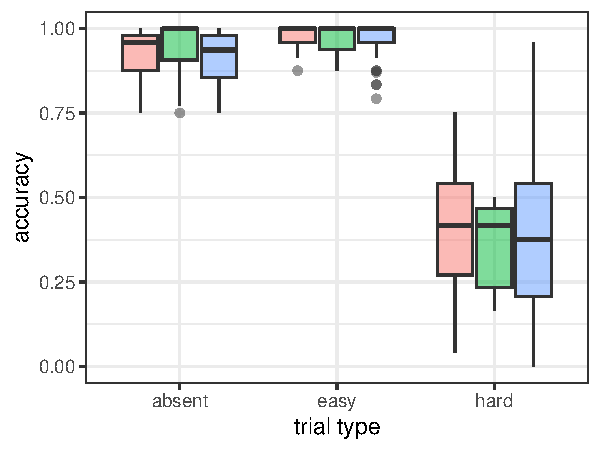
\includegraphics[width=6cm]{../analysis/scratch/acc_main.pdf}}
  \subfigure[]{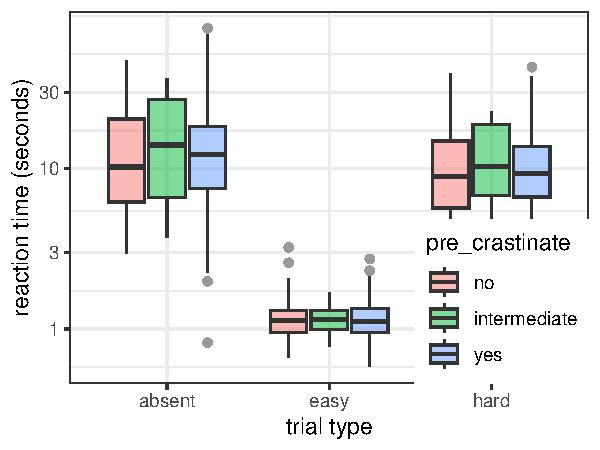
\includegraphics[width=6cm]{../analysis/scratch/rt_main.pdf}}
  \caption{The distribution of (a) accuracy and (b) reaction time measures in the split-half visual search task. Note that the $y$-axis for (b) has been $\log_2$-scaled. Dots represent points classed as outliers, defined as being below or above $1.5 \times$ the inter-quartile range away from the first or third quartile.}
  \label{fig:exp2_summary}
\end{figure}

\subsection{Pre-crastination}

The range of precrastination behaviours is shown in Figure (\ref{fig:exp2_strat_summary}(b). The majority of participants clearly either pre-crastinated (180, $59.0\%$) or not (105, $34.4\%$) with only a small minority (20, $6.5\%$) following an intermediate strategy. As such, we will treat pre-crastination as a two-level factor and exclude participants exhibiting intermediate behaviours. 

\begin{figure}[t]
  \centering  
  \subfigure[]{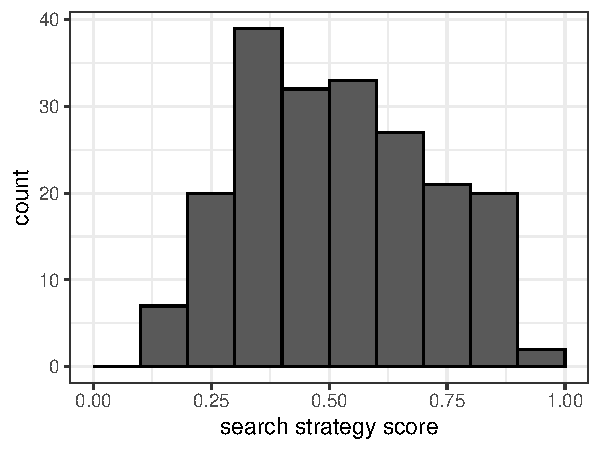
\includegraphics[width=6cm]{../analysis/scratch/strat_hist.pdf}}
  \subfigure[]{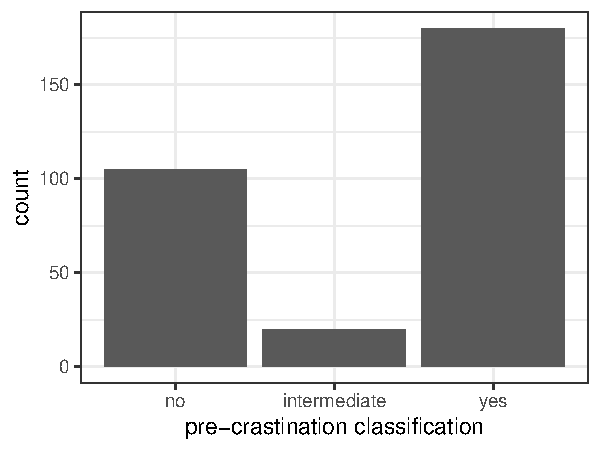
\includegraphics[width=6cm]{../analysis/scratch/pre_crastinate.pdf}}
  \caption{The distribution of (a) search strategy efficiency scores and (b) pre-crastination behaivours. We can see that there is a lot of variation in both measures. }
  \label{fig:exp2_strat_summary}
\end{figure}

\subsection{Planned Analysis}

The first step of our planned analysis is to test the hypothesis that there is a difference in  visual search strategy between those participants who pre-crastinated and those who did not. As registered, we fit a Bayesian beta regression model, the results of which are displayed in Figure \ref{fig:full_exp_strategy}. There is little-to-no evidence for a difference between the two groups, ($p(\delta >0| X)  =0.50$). This lack of differences makes hypothesis ii (that the effect size will be in line with the pilot data) redundant, but we report the $95\%$ HPDI $= [-0.0465, 0.0467$] for completeness sake.

\begin{figure}[t]
  \centering  


\subfigure[]{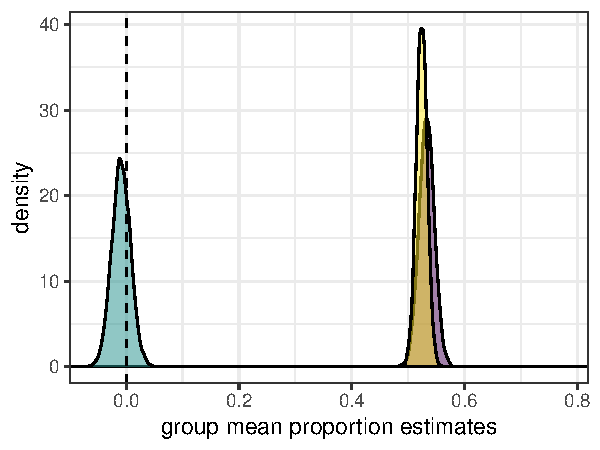
\includegraphics[width=6cm]{../analysis/scratch/post_plot.pdf}}
\subfigure[]{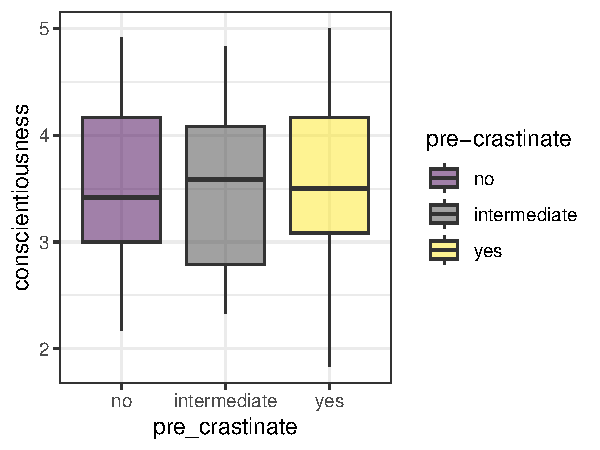
\includegraphics[width=6cm]{../analysis/scratch/pre_cras_consc.pdf}}
  \caption{(a) Posterior distributions for the mean of the two groups of participants, and the difference between them. (b) There is no evidence for a relationship between pre-crastination and conscientiousness}
  \label{fig:full_exp_strategy}
\end{figure}

Our final registered hypothesis concerns the relationship between pre-crastination and conscientiousness. We find no evidence for this relationship in our data. This holds whether we continue to treat pre-crastination as a binary variable ($95\%$ HPDI = [-0.19, 0.17] for the difference between groups) or as a continuous variable and measure the number of trials out of six in which participants pre-crastinated ($95\%$ HPDI = [-0.03, 0.03] for the effect of number of trials on conscientiousness).


\subsubsection{Discussion}

We met all outcome-neutral conditions and acquired a sample sufficient in size and quality to test the three hypotheses. As with the pilot data, the larger sample demonstated that precrastination behaviour is common, with more than half the participants picking up the close bucket first. We also replicated the wide range of variation between individuals in visual search effiency. We found no evidence for a consistent relationship between visual search effiency and precrastination, however, and no relationship between either measure and conscientiousness. Therefore, no evidence in favor of our registered hypotheses resulted from this experiment. 

\subsection{Exploratory Analysis}

We now investigate whether our data suggests any new hypotheses that could be of interest to other researchers.

\subsubsection{Personality and Visual Search Strategy}

\subsubsection{Personality and Pre-crastination}

\subsubsection{Other measures}

In addition to the registered measures, for efficiency we collected a range of other demographic characteristics and free-report measures from our participants. These are outside the scope of the pre-registration we have presented in this paper, so a full exploration of these additional variables and their relationship to visual search and precrastination will be presented elsewhere. In the interest of open science, however, and to avoid possible confusion by separating or duplicating data, the full set of data analysed in this pre-registration is presented along with these additional variables here: [link to data]. We request anyone wanting to use the data in this repository to contact the corresponding author and to reference... what? this paper? We'll need to write up a brief report about the data and submit it so people have something to reference. Maybe Anna could make a start on this??


\section{General Discussion}
Although the smaller pilot sample (N=30) suggested participants who pre-crastinate tended to use their peripheral vision to search more efficiently, the larger sample (N=201) did not support that conclusion. While this is a null finding, it is nonetheless meaningful because we had a clear prediction based on data and theory and designed a robust experiment to test it. We replicated the previously-established patterns in finding (1) a good split of people who consistently pre-crastinated and people who consistently did not and (2) a broad range of individual differences in visual search efficiency. If a stable relationship between these factors exists and is large enough to build any theories around, this experiment would have detected it. The fact that it did not detect it is useful in ruling out explanations for either behaviour (precrastination or visual search inefficiency) that is grounded in a shared personality characteristic like conscientiousness or impulsivity.

What did we learn?
The relationship between conscientiousness and pre-crastination observed previously was not observed here. We did have a rather conscientious sample though.
Possible relationships between procrastination and pre-crastiation is interesting and was also not observed previously.
People's reports of what they say they are doing / how they justify their choices is interesting and future research can explore these.
We have a rich dataset here with many other measures and we invite others to use it in hypothesis-generating exploratory analyses of their choosing.


\bibliographystyle{rs}
\small
\bibliography{literature.bib}

\end{document}

